\documentclass[12pt]{article}

\fontfamily{lmss}
\usepackage{fullpage}
\usepackage{amsmath}
\usepackage{amsthm}
\usepackage{url}
\usepackage{multicol}
\usepackage{enumerate}
\usepackage{graphicx}
\usepackage{color}
\usepackage{hyperref}
\hypersetup{
    colorlinks=true,
    linkcolor=blue,
    filecolor=magenta,      
    urlcolor=blue,
}

\usepackage{geometry}
\geometry{
  top=1in,            % <-- you want to adjust this
  bottom=1in,
  left=1in,
  right=1in,
  headheight=3ex,       % <-- and this
  headsep=4ex,          % <-- and this
}

\usepackage{lastpage}
\usepackage{fancyhdr}
\pagestyle{fancy}
\fancyhf{}
\renewcommand{\footrulewidth}{0.4pt}
\lhead{CS 486/686}
\rfoot{Page \thepage\ of \pageref{LastPage}}

\setlength{\parskip}{\baselineskip}%
\setlength{\parindent}{0pt}%

\usepackage{tcolorbox}
\tcbuselibrary{breakable}
\newenvironment{markscheme}
{
    \renewcommand{\parskip}{\baselineskip}
    \begin{tcolorbox}[
        colback=blue!10,
        colframe=blue!10,
        sharp corners,
        breakable
    ]
    \textbf{Marking Scheme:}
}
{
    \end{tcolorbox}
}

\newenvironment{sol}[1]{
\color{blue}
	{\bf Solution:}
}{
}

\newenvironment{problem}
{
    \begin{tcolorbox}[
        colback=green!15,
        colframe=green!15,
        sharp corners,
        breakable
    ]
    \setlength{\parskip}{1em}
    \textbf{Problem:}
}
{
    \end{tcolorbox}
}


\lfoot{\copyright Alice Gao 2021}
\chead{Spring 2021}
\rhead{Assignment 4}
\cfoot{v1.0}

\title{CS 486/686 Assignment 4 (90 marks)}
\author{Alice Gao}
\date{Due Date: 11:59 PM ET on Thursday, August 5, 2021
with an extension with no penalty to 11:59 pm ET on Wednesday, August 11, 2021}

\begin{document}

\maketitle

% \section*{Changes}

% \begin{itemize}
%     \item v1.1 Changed PDF so that question parts are labeled using a, b, ... instead of using 1 2, ...Updated Q1 problem description to clarify that host will choose randomly in step 2 if both doors have goats behind them.
% \end{itemize}

\newpage
\section*{Academic Integrity Statement}

{\color{red} If your written submission on Learn does not include this academic integrity statement with your signature (typed name), we will deduct 5 marks from your final assignment mark.}


I declare the following statements to be true:

\begin{itemize}
\item 
The work I submit here is entirely my own.

\item 	
I have not shared and will not share any of my code with anyone at any point. 

\item 
I have not posted and will not post my code on any public or private forum or website.

\item 	
I have not discussed and will not discuss the contents of this assessment with anyone at any point.

\item 
I have not posted and will not post the contents of this assessment and its solutions on any public or private forum or website. 

\item 
I will not search for assessment solutions online.

\item 
I am aware that misconduct related to assessments can result in significant penalties, possibly including failure in the course and suspension. This is covered in Policy 71: https://uwaterloo.ca/secretariat/policies-procedures-guidelines/policy-71.
\end{itemize}

Failure to accept the integrity policy will result in your assignment not being graded.

By typing or writing my full legal name below, I confirm that I have read and understood the academic integrity statement above.



\newpage
\section*{Instructions}

\begin{itemize}
\item
Submit the assignment in the A4 Dropbox on Learn. 
No late assignment will be accepted. This assignment is to be done individually.

\item 
I strongly encourage you to complete your write-up in Latex, using this source file. If you do, in your submission, please replace the author with your name and student number. Please also remove the due date, the Instructions section, and the Learning goals section. 
\item
Lead TAs: 
\begin{itemize}
\item
Niki Hasrati (\href{mailto:niki.hasrati@uwaterloo.ca}{niki.hasrati@uwaterloo.ca})
\end{itemize}
The TAs' office hours will be posted on MS Teams.
\end{itemize}



\section*{Learning goals}

{\bf Decision Networks}

\begin{itemize}
\item 
Model a real-world problem as a decision network with sequential decisions.
\item
Given a decision network with sequential decisions, determine the optimal policy and the expected utility of the optimal policy by applying the variable elimination algorithm.
\end{itemize}

{\bf Reinforcement Learning}
\begin{itemize}
\item
Implement the active adaptive dynamic programming algorithm for reinforcement learning.
\end{itemize}


\newpage
\section{Decision Network for ``Monty Hall'' (28 marks)}

The Monty Hall Problem is stated as follows.

You are on a game show, and you are given the choice of three doors: Behind one door is a car; behind the others, goats. The host knows what's behind each door but you don't.

\begin{enumerate}

\item 
First, you pick a door, say Door 1.

\item 
Second, the host opens another door, say Door 3, which has a goat behind it.

\item 
Finally, the host says to you, ``Do you want to pick Door 2?'' 
\end{enumerate}

Is it to your advantage to switch your choice in step 3? 

In step 2, the host always opens a door with a goat behind it, but not the door you chose first, regardless of which door you chose first. If both remaining doors have goats behind them, the host will open a door randomly. In step 3, you ``reserve'' the right to open the door you chose first, but can change to the remaining door after the host opens the door to reveal a goat. Your price is the item behind the final door you choose. You prefer cars over goats (cars are worth 1 and goats are worth 0). The car is behind doors 1, 2, and 3 with probabilities $p_1$, $p_2$ and $1 - p_1 - p_2$ respectively, and you know the values of $p_1$ and $p_2$.

Let's model this problem using the following variables.
    
\begin{itemize}

\item CarDoor $\in \{ 1, 2, 3\}$ is the door such that the car is behind it. This is a random variable.

\item FirstChoice $\in \{1, 2, 3\}$ is the index of the door you picked first. This is a decision variable.

\item HostChoice $\in \{smaller, bigger\}$ is the index of the door picked by the host. The value of this variable indicates whether the index of the door picked is the smaller or bigger one of the two doors left after you made your first choice. This is a random variable.
    
\item SecondChoice $\in \{stay, switch\}$ indicates whether you stay with the door you picked first or switch to the remaining door not opened by the host. This is a decision variable.

\item Utility $\in \{0, 1\}$ is 0 if you get a goat and 1 if you get a car. 

\end{itemize}


Please complete the following tasks.

\begin{enumerate}[(a)]

\item     
Complete the decision network in Figure~\ref{fig:monty_hall} by drawing all the arcs. Show the probability table for each random variable. Show the utility table for the utility node. You can use $p_1$ and $p_2$ in your tables since you do not know their values yet.

Hint: When you are deciding whether node A should be a parent of node B (a decision variable), think of the following. If node A is a parent of node B, then the optimal policy may be of a form that: if A has value a, then B should be b. Otherwise, if node A is not a parent of node B, the optimal policy for B cannot depend on the value of A. In other worlds, adding an edge in the network increases the set of possible policies that we would consider. 
    
\begin{figure}[ht!]
\centering
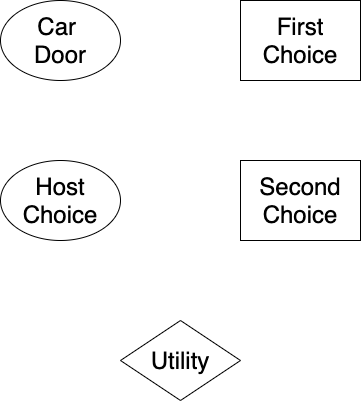
\includegraphics[width=0.4\textwidth]{images_posted/a4-dn1-empty.png}
\caption{The Monty Hall Problem}
\label{fig:monty_hall}
\end{figure}
    
\begin{markscheme}

(10 marks)

\begin{itemize}
    \item (4 marks) Correct parent nodes.
    \item (3 marks) Correct probability tables.
    \item (3 marks) Correct utility table.
\end{itemize}

\end{markscheme}


\item

{\bf Assume that $p_1 = 1/3$ and $p_2 = 1/3$.}  

Compute the optimal policy for the decision network by applying the variable elimination algorithm. Show all your work including all the intermediate factors created. Clearly indicate the optimal policy and the expected utility of the agent following the optimal policy.

\begin{markscheme}

(9 marks)

\begin{itemize}
    \item (4 marks) Sum out variables in the correct order.
    \item (2 marks) Correct optimal policy for FirstChoice.
    \item (2 marks) Correct optimal policy for SecondChoice.
    \item (1 mark) Correct value of the expected utility of the optimal policy.
\end{itemize}    

\end{markscheme}
    
    
\item

Consider a different case where {\bf $p_1 = 0.6$ and $p_2 = 0.25$.}  The car is much more likely to be behind door 1 than to be behind door 2 or 3. The car is slightly more likely to be behind door 2 than to be behind door 3.

Compute the optimal policy for the decision network by using the variable elimination algorithm. Show all your work including all the intermediate factors created. Clearly indicate the optimal policy and the expected utility of the agent following the optimal policy.

\begin{markscheme}

(9 marks)

\begin{itemize}
\item (4 marks) Sum out variables in the correct order.
\item (2 marks) Correct optimal policy for FirstChoice.
\item (2 marks) Correct optimal policy for SecondChoice.
\item (1 mark) Correct value of the expected utility of the optimal policy.
\end{itemize}    

\end{markscheme}
    
      
\end{enumerate}




\newpage
\section{Reinforcement Learning (62 marks)}

You will implement the {\bf adaptive dynamic programming} algorithm for reinforcement learning and use it to explore some grid worlds similar to the one discussed in lecture.

Section~\ref{sec:worlds} describes the grid worlds in our tests. Section~\ref{sec:active_adp} describes the active ADP algorithm in detail.

{\bf Please complete the following tasks.}

Implement all the empty functions in \verb+rl.py+. Submit \verb+rl.py+ only on Marmoset.

On Marmoset, we will verify the accuracy of the utilities returned by your implementation (\verb+actual_utilities+) using the code below.
%
\begin{verbatim}
np.allclose(correct_utilities, actual_utilities, atol=0.15)
\end{verbatim}
%
We derived the correct utilities by solving the Markov Decision Process using value iteration since we know the transition probabilities for each world. 

For any function that returns the utility values, make sure that the utility value of a wall is zero. Otherwise, you may fail our tests because of this.

\begin{markscheme}
(62 marks)

Unit tests
\begin{itemize}
\item \verb+get_transition_prob+

    (1 public test + 4 secret tests) * 1 mark = 5 marks

\item \verb+is_done_exploring+

    (1 public test + 4 secret tests) * 1 mark = 5 marks

\item \verb+get_best_action+

    (1 public test + 1 secret test) * 1 mark = 2 marks
    
\item \verb+exp_utils+

    (1 public test + 4 secret tests) * 2 marks = 10 marks

\item \verb+optimistic_exp_utils+

    (1 public test + 4 secret tests) * 1 mark = 5 marks

\item \verb+update_utils+

    (1 public test + 4 secret tests) * 2 marks = 10 marks

\item \verb+utils_to_policy+

    (1 public test + 4 secret tests) * 1 mark = 5 marks

\item \verb+adpa_move+

    (1 public test + 4 secret tests) * 2 marks = 10 marks
    
\item \verb+adpa+

    (1 public test + 4 secret tests) * 2 marks = 10 marks

\end{itemize}

\end{markscheme}

\subsection{The grid worlds}
\label{sec:worlds}

We will test your program on multiple grid worlds. Each world is provided in a file named \verb+world_*.txt+ where \verb+*+ is replaced by the world's name. As an example, we will provided the grid world discussed in lecture in \verb+world_lecture.txt+. The content of \verb+world_lecture.txt+ is shown below.
%
\begin{verbatim}
3,4
S * * *
* X * -1
* * * 1
1
-0.04
\end{verbatim}

The \verb+world_lecture.txt+ file provides the following information.
\begin{itemize}
    \item The first line describes the size of the grid. The first integer is the number of rows and the second integer is the number of columns.
    \item The next few lines describes the grid. \verb+S+ denotes the start state. \verb+X+ denotes a wall. Any integer value denotes a goal state with a reward equal to that integer. \verb+*+ denotes any other non-goal state.
    \item The next line gives the discount factor.
    \item The next line gives the immediate reward of entering any non-goal state.
\end{itemize}

For the \verb+lecture+ world, the transition probabilities are the same as the ones discussed in lecture. The agent moves in the intended direction with probability $0.8$, moves to the left of the intended direction with probability $0.1$, and moves to the right of the intended direction with probability $0.1$.

{\bf Any other grid world}

We may test your program with multiple other grid worlds. You can make the following assumptions regarding each grid world. 
\begin{itemize}
\item The world may not have the same dimensions as the \verb+lecture+ world.
\item The world has at least one goal state. Entering any goal state causes the agent to respawn in the start state.
\item The immediate reward of entering any non-goal state is a fixed float value and is provided in the \verb+world_*.txt+ file.
\item In each state, there are four available actions: up, right, down, and left. We encode them using integers: up: 0, right: 1, down: 2, left: 3. 
\item If the agent tries to move in a direction and hits a wall, the agent will stay in the same square.
\item 
By taking an action, the agent can end up traveling in any of the four directions with positive probability. 

In the \verb+lecture+ world, it is NOT possible for the agent to travel in the direction that is opposite of the intended direction. However, in other worlds, the agent may travel in an opposite direction of the intended direction with a positive probability. 
\end{itemize}

\newpage
\subsection{The Active Adaptive Dynamic Programming Algorithm}
\label{sec:active_adp}

Let's define some quantities that we will use in the active ADP algorithm.
\begin{itemize}

\item $\gamma$ is the discount factor. It's provided in the \verb+world_*.txt+ file.

\item $R(s)$ is the immediate reward of entering any non-goal state. This is provided in the \verb+world_*.txt+ file.

\item $N(s,a)$: the number of times that the agent has taken action $a$ in state $s$. This is a 3D numpy array as shown below.

\begin{verbatim}
n_sa = np.zeros((*grid.shape, num_actions))  
\end{verbatim}

\item $N(s,a,s')$: the number of times the agent has taken action $a$ in state $s$ and reached state $s'$. This is a 5D numpy array as shown below.

\begin{verbatim}
n_sas = np.zeros((*grid.shape, num_actions, *grid.shape))      
\end{verbatim}

\item $P(s'|s,a)$ is the probability of transitioning to state $s'$ if the agent executes action $a$ in state $s$. 
\item 
$N_e$ is an integer. It denotes the minimum number of times that the agent would like to explore any state-action pair. 

\item 
$R^+$ is an optimistic estimate of the reward if the agent hasn't taken action $a$ in state $s$ for at least $N_e$ times. 

$R^+$ should be set to a value that is greater than or equal to the maximum reward that the agent can obtain in any state.

\item $V^+(s)$: The optimistic estimates of the agent's expected utility of entering state $s$ and following the optimal policy thereafter. Use a 2D numpy array to store the long-term utility value for each state in the grid world.
\end{itemize}

The active ADP algorithm is described below.
\begin{enumerate}

\item 
Suppose that the current optimistic utility estimates be $V^+(s)$, the current state is $s$. Determine the agent's best action, denoted by $a$, as follows. 
%
\begin{align}
& \text{ best action } = \arg\max_a f \bigg( \sum_{s'} P(s'|s,a) V^+(s'), N(s,a) \bigg) \\
& f(u,n) = 
\begin{cases}
R^+, \text{ if } n < N_e \\
u, \text{ otherwise.}
\end{cases}
\end{align}

The quantity $f \bigg( \sum_{s'} P(s'|s,a) V(s'), N(s,a) \bigg)$ is the optimistic estimate of the expected utility of taking action $a$ in state $s$. 
%
If the agent has not taken action $a$ in state $s$ for at least $N_e$ times, this optimistic utility estimate is $R^+$. Otherwise, if the agent has taken action $a$ in state $s$ for at least $N_e$ times, the optimistic utility estimate is set to the actual utility estimate $\sum_{s'} P(s'|s,a) V(s')$.
%
In short, the optimistic utility estimate encourages the agent to try each state-action pair at least $N_e$ times.

{\bf We will rely on numpy to break ties.} Determine the best action using the code below, where \verb+opt_utils_for_a+ contains the four optimsitic utility estimates in the order up, right, down, and left.
\begin{verbatim}
np.argmax(opt_utils_for_a)    
\end{verbatim}

\item 
Carry out the best action $a$ computed in step 1 by calling the \verb+make_move_det+ function in \verb+rl_provided.py+. (The \verb+make_move_det+ function relies on the pre-generated random moves in the \verb+world_*_run.txt+ file.)

Suppose that taking action $a$ in state $s$ caused the agent to transition to state $s'$.

\item 
Increment the counts $N(s,a)$ and $N(s,a,s')$.
\begin{align*}
& N(s,a) = N(s,a) + 1 \\
& N(s,a,s') = N(s,a,s') + 1
\end{align*}
We will use these counts to estimate the transition probabilities.

\item 
Update these estimates by performing synchronous value iteration updates. Start with the optimistic utility estimates $V^+(s)$ from the previous iteration of the loop. Stop the value iteration updates when $V^+(s)$ converged based on the provided function \verb+utils_converged+ in \verb+rl_provided+.

The transition probability $P(s'|s, a)$ is calculated as follows:
\begin{align*}
P(s' | s, a) = 
\begin{cases}
0, \qquad\qquad \text{ if } N(s,a) = 0 \\
\displaystyle \frac{N(s,a,s')}{N(s,a)}, \text{ otherwise }
\end{cases}
\end{align*}

The value iteration updates are given below. 
\begin{align}
& V^+(s) \leftarrow R(s) + \gamma \max_{a} f \left( \sum_{s'} P(s'|s,a) V^+(s'), N(s,a) \right) \\
& f(u,n) = 
\begin{cases}
R^+, \text{ if } n < N_e \\
u, \text{ otherwise.}
\end{cases}
\end{align}


\item 
Repeat the steps above until both requirements below are satisfied. 

(1) The agent has visited each state-action pair $(s,a)$ at least $N_e$ times, and 

(2) The optimistic utility estimates $V^+(s)$ have converged based on the provided function \verb+utils_converged+.
\end{enumerate}
 
 
\newpage
\subsection{Testing Your Program}

In order to test your program, you will need to create a run file for each world. To do this, copy the contents of the \verb+world_*.txt+ into another file called \verb+world_*_secret.txt+ and add a last line describing the transition probabilities. See an example for the lecture world below.

\begin{verbatim}
3,4
S * * *
* X * -1
* * * 1
1
-0.04
0.8, 0.1, 0, 0.1
\end{verbatim}

The four transition probabilities should sum to 1. The meanings of the transition probabilities are as follows:
\begin{itemize}
\item The probability of traveling in the intended direction.
\item The probability of traveling 90 degrees clockwise to the intended direction.
\item The probability of traveling 180 degrees clockwise to the intended direction.
\item The probability of traveling 270 degrees clockwise to the intended direction.
\end{itemize}


To create the run file (for example, for a world you have defined in \verb+world_lecture_secret.txt+), run the script as follows.
%
\begin{verbatim}
python3 create_run.py -world_name lecture -num_samples 5000 -seed 0
\end{verbatim}
%

This will create a file called \verb+NEW_world_*_run.pickle+ which you will need to rename to \verb+world_*_run.pickle+. 

{\bf Important Note: If you run this script for the \verb+lecture+ world, the resulting \verb+run.pickle+ file will NOT match the provided \verb+world_lecture_run.pickle+ file.}

If your program crashes, you might want to generate a run file with a larger number of samples.

 
\end{document}





























